% chapter 4 section 1

\section{电场}

\subsection{电场}

\subsubsection{电荷}

物体的带电量称为电荷,日文中也可用電気量一词。其单位为库伦(C),且带电体间时常有满足库仑定律\footnote{诱电率$\varepsilon=\frac{1}{4k\pi}$}的作用力存在。
\begin{itembox}[l]{库仑定律}
    \begin{equation*}
        F=k\frac{Qq}{r^2}
    \end{equation*}
    \begin{itemize}
        \item $k=9\times10^9N\cdot m^2\cdot C^{-2}$
        \item 同性相斥,异性相吸
    \end{itemize}
\end{itembox}

\subsubsection{电场}

为了更方便得解释诸如重力、万有引力、电磁力等非接触力的作用方式,人们引入了“场” 的概念,并认为是场传递了各种各样的物理信息。因此在空间中传递上述库仑力的场即为\underline{电场},用单位电荷的受力定义。

\begin{figure}[p!]
    \centering
    \begin{minipage}[t]{0.48\textwidth}
        \centering
        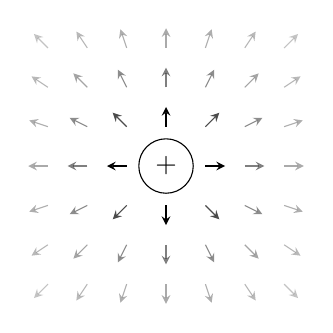
\begin{tikzpicture}[scale=0.5]
            \node[draw, circle] at (0,0) {$+$};
            \foreach \x in {-3,...,3} \foreach \y in {-3,...,3} {
                \pgfmathparse{and(equal(\x,0),equal(\y,0))}
                \ifnum\pgfmathresult=1
                \else
                \draw[-stealth, opacity={1/sqrt((\x)^2+(\y)^2)}] (\x,\y) -- ++ (
                    {0.5*\x/sqrt((\x)^2+(\y)^2)},
                    {0.5*\y/sqrt((\x)^2+(\y)^2)}
                );
                \fi
            }
        \end{tikzpicture}
        \caption{单正点电荷电场图示}
    \end{minipage}
    \begin{minipage}[t]{0.48\textwidth}
        \centering
        \begin{tikzpicture}[scale=0.5]
            \node[draw, circle] at (0,0) {$-$};
            \foreach \x in {-3,...,3} \foreach \y in {-3,...,3} {
                \pgfmathparse{and(equal(\x,0),equal(\y,0))}
                \ifnum\pgfmathresult=1
                \else
                \draw[-stealth, opacity={1/sqrt((\x)^2+(\y)^2)}] ($(\x,\y)+(
                    {0.5*\x/sqrt((\x)^2+(\y)^2)},
                    {0.5*\y/sqrt((\x)^2+(\y)^2)}
                )$) -- (\x,\y);
                \fi
            }
        \end{tikzpicture}
        \caption{单负点电荷电场图示}
    \end{minipage}
\end{figure}

\begin{figure}[p!]
    \centering
    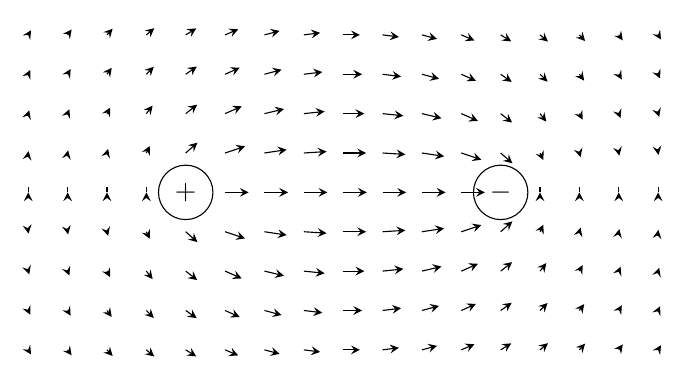
\begin{tikzpicture}[scale=0.5]
        \node[draw, circle] at (-4,0) {$+$};
        \node[draw, circle] at (4,0) {$-$};
        \foreach \x in {-8,...,8} \foreach \y in {-4,...,4} {
            \pgfmathparse{or(
                and(equal(\x,-4),equal(\y,0)),
                and(equal(\x,4),equal(\y,0))
            )}
            \ifnum\pgfmathresult=1
            \else
            \draw[-stealth] (\x,\y) -- ++ (
                {0.3*((\x+4)/sqrt((\x+4)^2+(\y)^2)-(\x-4)/sqrt((\x-4)^2+(\y)^2))},
                {0.3*(\y/sqrt((\x+4)^2+(\y)^2)-\y/sqrt((\x-4)^2+(\y)^2))}
            );
            \fi
        }
    \end{tikzpicture}
    \caption{正-负点电荷电场图示}
\end{figure}

\begin{figure}[p!]
    \centering
    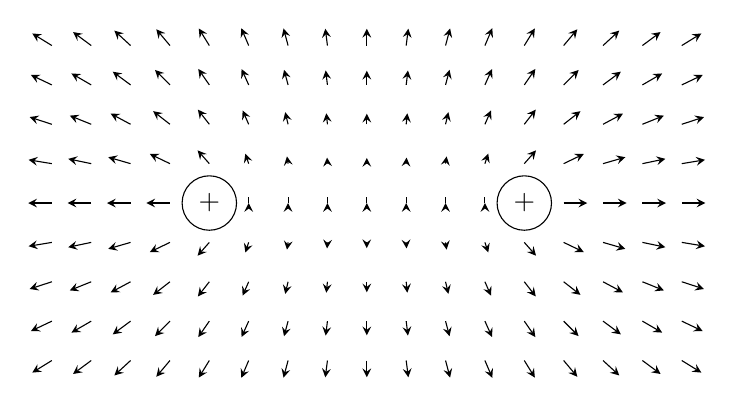
\begin{tikzpicture}[scale=0.5]
        \node[draw, circle] at (-4,0) {$+$};
        \node[draw, circle] at (4,0) {$+$};
        \foreach \x in {-8,...,8} \foreach \y in {-4,...,4} {
            \pgfmathparse{or(
                and(equal(\x,-4),equal(\y,0)),
                and(equal(\x,4),equal(\y,0))
            )}
            \ifnum\pgfmathresult=1
            \else
            \draw[-stealth] (\x,\y) -- ++ (
                {0.3*((\x+4)/sqrt((\x+4)^2+(\y)^2)+(\x-4)/sqrt((\x-4)^2+(\y)^2))},
                {0.3*(\y/sqrt((\x+4)^2+(\y)^2)+\y/sqrt((\x-4)^2+(\y)^2))}
            );
            \fi
        }
    \end{tikzpicture}
    \caption{正-正点电荷电场图示}
\end{figure}

\begin{itembox}[l]{电场}
    \begin{equation*}
        \vec{E}=\frac{\vec{F}}{q}
        \iff
        \vec{F}=q\vec{E}
    \end{equation*}
    \begin{itemize}
        \item 单位:N/C
        \item 点电荷周围的电场:$E=k\frac{Q}{r^2}$
    \end{itemize}
\end{itembox}
根据定义可知电场也是一个矢量,所以在实际运用过程中也满足矢量的合成与分解。

\subsection{电势}

\subsubsection{电势能与电势}

观察库仑力形式可发现其与万有引力十分相像,因此不难推测库仑力也是保存力。因而也有其对应的势能,即\underline{电势能},日文为静電気力による位置エネルギー。

此外,为了描述物理现象与计算使用方便,人们也引入了电场中单位电荷的电势能:电势(日文为電位)这个物理量,单位为伏特(V)。因此,电势能与电势之间满足如下关系。
\begin{itembox}[l]{电势能与电势}
    \begin{equation*}
        U=qV
    \end{equation*}
\end{itembox}

\subsubsection{典型电场中的电势}

\paragraph{匀强电场的电势}日文为一様電場,即大小、方向均衡定的电场。
\begin{figure}[ht!]
    \centering
    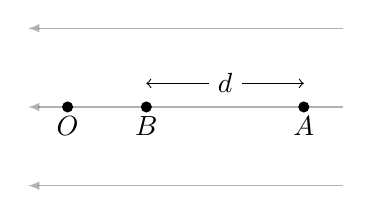
\begin{tikzpicture}
        \foreach \y in {0,1,2} {\draw[opacity=0.3, -latex] (4,\y) -- (0,\y);}
        \fill (0.5,1) circle (2pt) node[below] {$O$};
        \fill (1.5,1) circle (2pt) node[below] {$B$};
        \fill (3.5,1) circle (2pt) node[below] {$A$};
        \draw[<->] (1.5,1.3) -- node[fill=white] {$d$} (3.5,1.3);
    \end{tikzpicture}
    \caption{匀强电场电势}
\end{figure}
那么,匀强电场中倘若某两点间距为$d$,期间将会存在
\begin{equation*}
    V=\frac{Eq\times d}{q}=Ed
\end{equation*}
大小的电势,并称其为该两点间的\underline{电势差}。

\paragraph{点电荷电场的电势}

规定离场源电荷无限远处为电势基准,则可得点电荷周围电势公式。
\begin{itembox}[l]{点电荷电势}
    \begin{equation*}
        U=k\frac{kQ}{r}
    \end{equation*}
\end{itembox}

\subsubsection{等电势面}

类比于地图上描述地势分布的等高线,等电势线/面也常常用于描述电势的分布,且具有如下性质。
\begin{itemize}
    \item 与电场线垂直
    \item 等电位面密$\iff$电场线密$\iff$电场强
\end{itemize}
\begin{figure}[ht!]
    \centering
    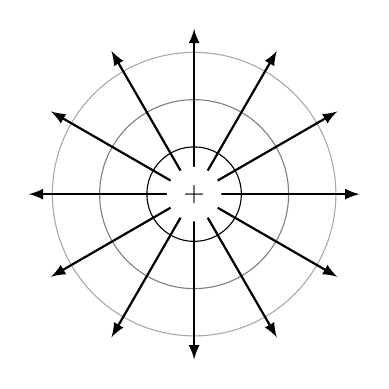
\begin{tikzpicture}[scale=0.6]
        \foreach \r in {1,...,3} {\draw[opacity={1/\r}] (0,0) circle (\r);}
        \foreach \a in {1,...,12} {\draw[thick, -latex] (0,0) -- ({\a*30}:3.5);}
        \node[circle, fill=white] at (0,0) {$+$};
    \end{tikzpicture}
    \caption{等电位面}
\end{figure}

\subsubsection{总结}

鉴于本节内容较多且不易梳理清晰,特此简做总结。
\begin{figure}[ht!]
    \centering
    \renewcommand\arraystretch{1.5}
    \begin{tabular}{c|c|c|c|c}
        \hline
        &电场E&库仑力F&电势能U&电势V\\\hline
        重力场&$g$&$mg$&$mgh$&$gh$\\\hline
        点电荷&$\frac{kQ}{r^2}$&$\frac{kQq}{r^2}$&$\frac{kQq}{r}$&$\frac{kQ}{r}$\\\hline
    \end{tabular}
    \caption{电场电势总结}
\end{figure}

\subsection{电容器}

\textbackslash\textbackslash TODO
